\documentclass[11pt,a4paper]{article}

\usepackage[utf8]{inputenc}
\usepackage[T1]{fontenc}
\usepackage{lmodern}
\usepackage[margin=2.3cm]{geometry}
\usepackage{amsmath,amssymb,bm}
\usepackage{mhchem}
\usepackage{siunitx}
\usepackage{graphicx}
\usepackage{booktabs,tabularx}
\usepackage{enumitem}
\usepackage[dvipsnames]{xcolor}
\usepackage{tcolorbox}
\usepackage{tikz}
\usetikzlibrary{arrows.meta,positioning,shapes.geometric}
\usepackage{listings}
\usepackage{microtype}
\usepackage[colorlinks=true,linkcolor=MidnightBlue,citecolor=ForestGreen,urlcolor=MidnightBlue]{hyperref}

\sisetup{detect-all}
\lstset{basicstyle=\ttfamily\small,columns=fullflexible,keepspaces=true,
        frame=single,framerule=0.3pt,rulecolor=\color{gray!60},backgroundcolor=\color{gray!6}}

\newtcolorbox{keybox}[1]{colback=MidnightBlue!4,colframe=MidnightBlue!70,
  fonttitle=\bfseries,title=#1,boxrule=0.6pt,arc=2pt}
\newtcolorbox{warnbox}[1]{colback=BrickRed!4,colframe=BrickRed!70,
  fonttitle=\bfseries,title=#1,boxrule=0.6pt,arc=2pt}
\newtcolorbox{nowbox}[1]{colback=ForestGreen!4,colframe=ForestGreen!70,
  fonttitle=\bfseries,title=#1,boxrule=0.6pt,arc=2pt}
\newcommand{\question}[1]{\par\smallskip\noindent\textcolor{MidnightBlue}{\textbf{Q.}~\emph{#1}}\par\smallskip}

\title{\textbf{A neural network potential for the Zundel ion}\\[4pt]
\large Lesson notes accompanying \texttt{tutorial\_01\_zundel/zundel.ipynb}}
\author{Machine-learned interatomic potentials --- hands-on session}
\date{}

\begin{document}
\maketitle

\begin{abstract}
These notes go with the first notebook of the MLIP tutorial. You will build a
machine-learned interatomic potential (MLIP) from start to finish: reference
data, descriptors, a neural network, active learning by \emph{query by
committee}, production molecular dynamics (MD) in CP2K, and validation against
the reference. The system is deliberately tiny: one \ce{H5O2+} ion in vacuum,
two chemical elements, a semi-empirical reference method and a network with
ten hidden neurons. It is a \textbf{basic, pedagogical example}. Every step is
the same one you would take in a research project, but every number is chosen
so that the whole workflow runs on a laptop in a few minutes. The last section
lists the subtleties that can be added on top of this simple model, and how
you would tackle the same problem in a research setting.
\end{abstract}

\tableofcontents

%======================================================================
\section{Why machine-learned potentials?}
%======================================================================

An MD simulation integrates Newton's equations
$m_i\ddot{\mathbf r}_i = \mathbf F_i = -\nabla_{\mathbf r_i}E(\{\mathbf r\})$.
Everything depends on the potential energy surface (PES) $E(\{\mathbf r\})$,
and there are two traditional ways to get it:
\begin{itemize}[nosep]
  \item \textbf{Electronic structure} (DFT, quantum chemistry, or here
        DFTB). It is accurate and reactive, but costs roughly $\mathcal O(N^3)$
        or more per step. This limits you to $\sim 10^2$--$10^3$ atoms and
        tens of picoseconds.
  \item \textbf{Empirical force fields}. They cost $\mathcal O(N)$ and are
        very fast, but have a fixed functional form. They usually cannot break
        bonds and are only as accurate as their parametrisation.
\end{itemize}
An MLIP is a flexible regression model $E_\theta(\{\mathbf r\})$ fitted to
reference electronic-structure energies and forces. It has the
$\mathcal O(N)$ cost of a force field, and \emph{within the region of
configuration space covered by its training data} it reaches the accuracy of
the reference. The italicised part is the whole difficulty, and it is the
thread running through this tutorial.

\begin{keybox}{What this example is --- and what it is not}
\begin{tabularx}{\linewidth}{@{}lX@{}}
\textbf{System} & One \ce{H5O2+} ion (7 atoms) in vacuum, no periodic boundaries.\\
\textbf{Reference} & SCC-DFTB, NVT at \SI{300}{K}, \SI{25}{ps} trajectory. Cheap, but \emph{not} a high-accuracy method.\\
\textbf{Model} & 2nd-generation Behler--Parrinello network~\cite{Behler2007}: one $28/32 \to 5 \to 5 \to 1$ network per element, about 380 weights in total.\\
\textbf{Training} & n2p2~\cite{Singraber2019} (Kalman filter), driven by the \texttt{aml} package~\cite{Schran2020}.\\
\textbf{MD} & CP2K~\cite{Kuhne2020}, NNP force environment.\\
\end{tabularx}
\medskip
Research-grade MLIPs are trained on DFT or coupled-cluster data, for
condensed phases with thousands of atoms, often with many elements. They use
much larger (often equivariant, message-passing) models, or start from a
pretrained foundation model (Sec.~\ref{sec:novelty}). The \emph{concepts} you
practise here --- locality, descriptors, committees, active learning,
validation by observables, transferability --- carry over unchanged.
\end{keybox}

%======================================================================
\section{The system and the reference data}
%======================================================================

The Zundel ion \ce{H5O2+} is an excess proton shared between two water
molecules, \ce{[H2O\bond{...}H\bond{...}OH2]+}. Together with the Eigen
cation \ce{H9O4+} it is one of the two limiting structures of the hydrated
proton. It is central to the Grotthuss mechanism of proton transport in
water~\cite{Marx1999}. Its PES is strongly anharmonic: the shared proton moves
in a very flat, nearly symmetric potential along the O--O axis. Even this
small cluster is therefore a non-trivial test for a potential.

\paragraph{Reference trajectory (\texttt{data/}).}
\begin{itemize}[nosep]
  \item Method: self-consistent-charge DFTB~\cite{Elstner1998} in CP2K, total charge $+1$.
  \item Ensemble: NVT, \SI{300}{K}, CSVR thermostat~\cite{Bussi2007} ($\tau=\SI{200}{fs}$), $\Delta t = \SI{0.5}{fs}$, \num{50000} steps (\SI{25}{ps}).
  \item Output every 5 steps: \num{10001} frames, \SI{2.5}{fs} apart, with positions, \emph{forces} and velocities, plus the energy file \texttt{zundel-1.ener}.
  \item Centre-of-mass translation and rotation are removed.
\end{itemize}
Every frame is a labelled data point $(\{\mathbf r\}, E, \{\mathbf F\})$.
One structure with 7 atoms gives 1 energy but 21 force components, so the
forces carry most of the information.

\question{Consecutive frames are only \SI{2.5}{fs} apart. How many of the
10\,001 frames are really \emph{independent}? What does that imply for a
random train/test split?}

%======================================================================
\section{The Behler--Parrinello neural network potential}
%======================================================================

\subsection{Locality: energy as a sum of atomic energies}
The central approximation of almost all MLIPs is \emph{locality}. The total
energy is a sum of atomic contributions, and each one depends only on the
neighbours within a cutoff radius $r_c$:
\begin{equation}
  E(\{\mathbf r\}) = \sum_{i=1}^{N} E_{Z_i}\!\left(\mathbf G_i\right),
  \qquad
  \mathbf F_j = -\sum_i \frac{\partial E_{Z_i}}{\partial \mathbf G_i}\cdot
                 \frac{\partial \mathbf G_i}{\partial \mathbf r_j}.
  \label{eq:hdnnp}
\end{equation}
$E_{Z}$ is a feed-forward network, one per chemical element $Z$, shared by all
atoms of that element. The construction makes the cost linear in $N$ and the
model size-extensive: you can, in principle, apply it to a larger system
(Sec.~\ref{sec:transfer}). The forces are \emph{exact} derivatives of the
energy, so the model is conservative by design.

\subsection{Descriptors: atom-centred symmetry functions}
The input $\mathbf G_i$ must be invariant under translation, rotation and
permutation of identical atoms. Behler--Parrinello models use
atom-centred symmetry functions (ACSFs)~\cite{Behler2011}. With the cosine
cutoff $f_c(r) = \tfrac12\left[\cos(\pi r/r_c)+1\right]$ for $r<r_c$:
\begin{align}
  G^{\mathrm{rad}}_i &= \sum_{j\neq i} e^{-\eta (r_{ij}-r_s)^2} f_c(r_{ij}),\\
  G^{\mathrm{ang}}_i &= 2^{1-\zeta}\sum_{j,k\neq i}
     \left(1+\lambda\cos\theta_{ijk}\right)^{\zeta}
     e^{-\eta(r_{ij}^2+r_{ik}^2+r_{jk}^2)}
     f_c(r_{ij})f_c(r_{ik})f_c(r_{jk}).
\end{align}
Each function is resolved by the elements of the neighbours, so there are
separate functions for O--O and O--H pairs, and for each neighbour pair in the
angular terms. The \texttt{aml} default set used in the notebook has:
\begin{itemize}[nosep]
  \item cutoff $r_c = 12\,a_0 \approx \SI{6.35}{\angstrom}$, which covers the whole ion;
  \item 10 radial functions per element pair, with Gaussians shifted between
        \SI{0.5}{\angstrom} and $r_c-\SI{0.5}{\angstrom}$;
  \item 4 angular functions per triple ($\lambda=\pm1$, $\zeta=1,4$, centred);
  \item the O--O--O triple excluded (\texttt{exclude\_triples}), since the ion has only two oxygens.
\end{itemize}
This gives 28 descriptors for O and 32 for H. You can plot them
with
\texttt{aml.acsf.plot\_radial} and \texttt{aml.acsf.plot\_angular}.

\subsection{Network and training}
The notebook defines each element network in \texttt{input.nn} through
\texttt{set\_nn()}: 2 hidden layers of 5 neurons, $\tanh$ activations and a
linear output (\texttt{t t l}). That is 181 weights for O and 201 for H.
n2p2 fits energies \emph{and} forces with a (global) extended Kalman
filter~\cite{Singraber2019b}, a second-order optimiser that is very efficient
for small networks. 10\,\% of the structures are held out as a test set, and
the \texttt{learning-curve.out} files record the train/test RMSE per epoch.

\begin{warnbox}{Units}
\texttt{aml} works internally in atomic units (Hartree, Bohr). The notebook
converts with $1\,E_h/a_0 = \SI{51.422}{eV/\angstrom}$ and
$1\,E_h = \SI{27.211}{eV}$. Force errors are usually quoted in
\si{meV/\angstrom}.
\end{warnbox}

%======================================================================
\section{A naive first model}
%======================================================================

The first experiment trains a \emph{single} network on every 25th frame of the
reference trajectory: 401 structures, evenly spaced in time, for 50 epochs.
The test errors look reasonable. You then run MD with this model
(\texttt{single/}, \SI{50}{ps}).

In a test run of this notebook, the dynamics stayed stable for about
\SI{4.9}{ps}. The temperature then jumped above \SI{1000}{K}, reached
$\sim\!10^{5}\,$K, and the ion dissociated: the O--O distance, which stays
between 2.2 and \SI{2.7}{\angstrom} in the reference, grew to
$\sim\!\SI{100}{\angstrom}$. The details change from run to run (random
initial weights, random train/test split), but a failure of this kind is
typical.

\paragraph{Why?} The MD trajectory has wandered into a region of configuration
space the training set did not cover: a rare, high-energy fluctuation of the
shared proton or of the O--O distance. There the network \emph{extrapolates}.
A neural network has no physical prior, so it can predict an unphysical hole
in the PES that pulls atoms together, or a spurious force that pumps in
energy. Once the system enters such a region, the error feeds on itself.

\begin{keybox}{Lesson 1: a low test RMSE does not guarantee stable MD}
The test set comes from the same distribution as the training set, so it
cannot detect holes outside that distribution. MD finds them, because it
explores configuration space systematically, including its rare-event
tails. This observation has since been documented
systematically~\cite{Fu2022}. Always validate a potential by \emph{running}
it.
\end{keybox}

\question{Evenly spaced frames sample configurations by their Boltzmann
weight. Which configurations are therefore under-represented, and why are they
exactly the dangerous ones?}

%======================================================================
\section{Committees and query by committee}
%======================================================================

\subsection{The committee as an uncertainty estimate}
Instead of one network, train a \emph{committee} of $n$ networks
(here $n=8$). They differ in initial weights, in the random train/test split
and in the order of the stochastic updates~\cite{Schran2020}. The prediction
is the committee mean, and the spread is an uncertainty estimate:
\begin{equation}
  \bar E = \frac1n\sum_{k=1}^n E^{(k)},\qquad
  \sigma_E = \sqrt{\frac1{n}\sum_{k=1}^n \left(E^{(k)}-\bar E\right)^2},
\end{equation}
and likewise for every force component. Where training data exist, the members
agree. Away from the data each one extrapolates differently, and
$\sigma$ grows. A large committee disagreement is not an error bar in the
strict statistical sense, but it is a cheap and remarkably useful indicator of
\emph{"this configuration is outside what I know"}.

\subsection{Active learning: query by committee (QbC)}
\emph{Query by committee}~\cite{Seung1992} uses the disagreement to choose
training data. The notebook applies it to an existing pool (the full
10\,001-frame reference trajectory), so no new reference calculations are
needed:

\begin{center}
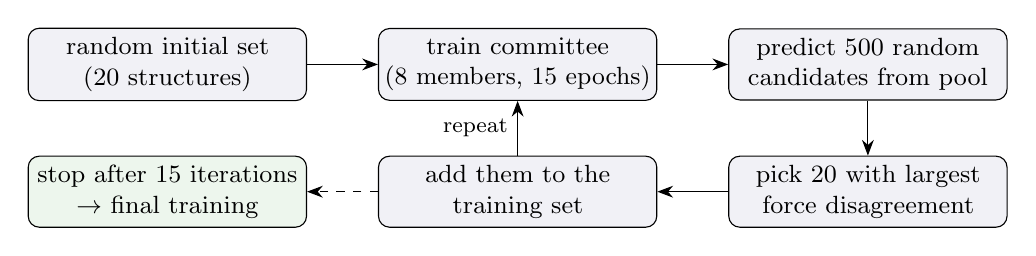
\begin{tikzpicture}[node distance=7mm and 9mm,
  box/.style={draw,rounded corners,fill=MidnightBlue!6,align=center,
              minimum height=9mm,text width=33mm,font=\small},
  >={Stealth[length=2mm]}]
  \node[box] (init) {random initial set\\(20 structures)};
  \node[box,right=of init] (train) {train committee\\(8 members, 15 epochs)};
  \node[box,right=of train] (pred) {predict 500 random\\candidates from pool};
  \node[box,below=of pred] (sel) {pick 20 with largest\\force disagreement};
  \node[box,left=of sel] (add) {add them to the\\training set};
  \node[box,left=of add,fill=ForestGreen!8] (stop) {stop after 15 iterations\\$\to$ final training};
  \draw[->] (init) -- (train);
  \draw[->] (train) -- (pred);
  \draw[->] (pred) -- (sel);
  \draw[->] (sel) -- (add);
  \draw[->] (add) -- node[left,font=\footnotesize]{repeat} (train);
  \draw[->,dashed] (add) -- (stop);
\end{tikzpicture}
\end{center}

\noindent
For each candidate, \texttt{aml} computes the committee standard deviation of
every force component. The structure is then scored by a high-order
(6th) moment of these values, which emphasises the single worst atom rather
than the average. After 15 iterations the training set holds at most
$20+15\times20 = 320$ structures, \emph{fewer} than the 401 of the naive
model. The final model is a fresh 8-member committee, trained for 50 epochs
on this set (\texttt{train/final\_training}).

The notebook prints three disagreements at every iteration: on the training
set, on the random candidates, and on the selected structures. Track how they
evolve. In a test run (Table~\ref{tab:qbc}), the disagreement on the
candidates fell by a factor of $\sim\!20$ over 15 iterations. Late
iterations started re-selecting structures already in the set, a sign of
convergence. The final model was trained on 284 structures.

\begin{table}[h]
\centering\small
\caption{Mean committee force disagreement (\si{meV/\angstrom}) during QbC
in a test run. Your numbers will differ (random sampling and weights); the
trend will not.}
\label{tab:qbc}
\begin{tabular}{@{}rrrrr@{}}
\toprule
iteration & training-set size & train & candidates & selected\\
\midrule
1  & 20  & 307 & 695 & 5609\\
2  & 40  & 152 & 151 & 289\\
3  & 60  & 111 &  95 & 139\\
5  & 100 &  85 &  70 & 108\\
10 & 194 &  62 &  47 &  68\\
15 & 284 &  51 &  37 &  56\\
\bottomrule
\end{tabular}
\end{table}

\question{Is the disagreement on the training set always the smallest? Check
Table~\ref{tab:qbc}: from iteration 2 on it is \emph{larger} than on random
candidates. Why? (Think about which structures the training set is made of.)
Why do the selected structures sit preferentially at \emph{high} potential
energy along the trajectory (plot of training points vs.\ $E_p(t)$)?}

\question{How does the wall time of one QbC iteration grow with the iteration
index? (In the test run it barely changed, 11--\SI{12}{s}: for such small sets
the fixed costs dominate.) Which part of the work scales with the training-set size, and which
with the committee size?}

\begin{keybox}{Lesson 2: not all configurations are equally valuable}
A thermal trajectory is extremely redundant. Active learning spends the
reference-data budget on the configurations the model is most uncertain about.
This gives a smaller and better training set, and in production it lets the
uncertainty be monitored on the fly.
\end{keybox}

%======================================================================
\section{Production MD and validation}
%======================================================================

\subsection{Running the committee in CP2K}
\texttt{N2P2.save\_model()} writes one directory \texttt{nnp-XXX} per member.
The CP2K input loads all of them:
\begin{lstlisting}
@SET PATH ../train/final_training/model
&NNP
  NNP_INPUT_FILE_NAME ${PATH}/nnp-000/input.nn
  SCALE_FILE_NAME     ${PATH}/nnp-000/scaling.data
  &MODEL
    WEIGHTS ${PATH}/nnp-000/weights
  &END MODEL
  ...                       # one &MODEL block per member
&END NNP
\end{lstlisting}
CP2K propagates the dynamics with the committee mean. The
\texttt{\&PRINT/\&ENERGIES} section writes the energy of every member, from
which you get the committee disagreement along the trajectory. The cost grows linearly with the number
of members. If you change \texttt{n\_members}, edit the \texttt{\&MODEL}
blocks to match.

\subsection{Validation by observables}
Low force errors are necessary but not sufficient, so the notebook compares
\emph{simulation observables} between the NNP and DFTB trajectories with
\texttt{aml.score}:
\begin{itemize}
  \item \textbf{Radial distribution functions} $g_{\alpha\beta}(r)$ for the
        O--O, O--H and H--H pairs (structure).
  \item \textbf{Vibrational density of states}, computed from the velocity
        autocorrelation function,
        $I(\omega)\propto\int \sum_i\langle\mathbf v_i(0)\cdot\mathbf v_i(t)\rangle
        \,w(t)\,e^{-i\omega t}\,dt$, with a Hann window $w$ (dynamics).
        The O--H stretch region near \SI{3000}{cm^{-1}} and the low-frequency
        shared-proton modes are the sensitive parts.
\end{itemize}
For each curve the score is a normalised absolute deviation,
$\varepsilon = \sum|f_{\mathrm{ref}}-f_{\mathrm{NNP}}| /
\left(\sum f_{\mathrm{ref}}+\sum f_{\mathrm{NNP}}\right)$, where 0 means
identical, and \texttt{aml} prints $100\,(1-\varepsilon)$ as an
``accuracy'' in \%. In the test run, the final committee ran \SI{50}{ps}
without problems: the temperature stayed below \SI{750}{K}, as in the
reference, and the O--O distance stayed in 2.22--\SI{2.63}{\angstrom}
(reference 2.24--\SI{2.69}{\angstrom}). The scores were \SI{95.8}{\%} for
the RDFs (O--O \SI{92.8}{\%}, O--H \SI{97.0}{\%}, H--H \SI{97.5}{\%}) and
\SI{90.6}{\%} for the VDOS.

\question{Why is the O--O RDF error typically the largest? (Count how many O--O
pairs contribute to the histogram.) Is it surprising to reach good agreement
for a single molecule?}

%======================================================================
\section{Transferability: a bigger cluster}
\label{sec:transfer}
%======================================================================

Thanks to Eq.~\eqref{eq:hdnnp}, nothing stops you from running the same
model on \ce{(H2O)6H+} (\texttt{cluster/}, \SI{500}{fs}). Running it is
technically possible; getting it right is not guaranteed. The larger cluster
contains environments the Zundel ion never had:
\begin{itemize}[nosep]
  \item water--water hydrogen bonds that do not involve the excess proton;
  \item more neighbours inside the cutoff, so descriptor values fall
        outside the range seen in training (\texttt{scaling.data} records
        that range);
  \item O--O--O triples, whose angular terms were \emph{excluded} from the model.
\end{itemize}
In the test run the temperature exceeded \SI{1000}{K} within the first
femtoseconds and reached $\sim\!10^5\,$K: the model fails immediately. Use
the committee disagreement to diagnose such failures. This motivates the second tutorial (\texttt{wclusters.ipynb}), which
trains on the larger cluster and probes transfer to a 17-water cluster and to
bulk water.

\begin{keybox}{Lesson 3: an MLIP knows only what it has seen}
Locality makes a model \emph{applicable} to new systems; only training data
make it \emph{reliable} there. Transferability must be tested, never assumed.
And the model can never be better than its reference: as tutorial~2 shows,
this DFTB parametrisation gives heavily over-structured liquid water.
\end{keybox}

%======================================================================
\section{Going further: subtleties beyond the simple model}
\label{sec:novelty}
%======================================================================

The workflow above --- Behler--Parrinello networks, ACSFs, committee-based
active learning --- is deliberately simple, and perfectly valid. It is a
very good way to \emph{understand} MLIPs. Each of its ingredients can be
refined, and the subtleties below are the main ones a practitioner would add
on top of it.

\subsection{Architectures: from fixed descriptors to equivariant message passing}
\begin{itemize}
  \item \textbf{Systematic many-body descriptors.} The atomic cluster expansion
        (ACE)~\cite{Drautz2019} provides a complete, systematically improvable
        basis that replaces hand-chosen ACSF sets.
  \item \textbf{Equivariant message-passing networks.} NequIP~\cite{Batzner2022},
        Allegro~\cite{Musaelian2023} and MACE~\cite{Batatia2022} learn the
        representation instead of fixing it. They propagate geometric
        (tensorial) features that rotate with the structure, and capture
        many-body correlations efficiently. They are markedly more
        data-efficient than descriptor-based networks: a few hundred
        structures can be enough where thousands were needed
        before~\cite{Batzner2022}.
  \item \textbf{Long-range interactions.} The strict cutoff in
        Eq.~\eqref{eq:hdnnp} misses electrostatics and charge transfer, which
        matters for an \emph{ion} like \ce{H5O2+}. Fourth-generation
        networks~\cite{Ko2021} learn environment-dependent charges with a
        global charge equilibration. Latent Ewald summation~\cite{Cheng2024}
        adds a learned long-range term without reference charges.
  \item \textbf{Conservative vs.\ direct forces.} Some large models
        predict forces directly instead of as $-\nabla E$, for speed. This was
        shown to cause drift and instabilities in MD~\cite{Bigi2024}, so
        conservative forces are preferred, at least for
        simulation~\cite{Fu2025}. The Behler--Parrinello model you train here
        is conservative by construction.
\end{itemize}

\subsection{Foundation (universal) models}
Instead of fitting \emph{one potential per system} from scratch, as done
here, one can start from a \emph{pretrained general-purpose potential}:
\begin{itemize}
  \item \textbf{Materials.} MACE-MP-0~\cite{Batatia2023}, trained on the
        Materials Project relaxation trajectories, runs stable MD for most of
        the periodic table out of the box. Meta's OMat24~\cite{BarrosoLuque2024}
        dataset ($>10^8$ DFT calculations) and the models trained on it pushed
        accuracy further.
  \item \textbf{Molecules.} MACE-OFF~\cite{Kovacs2023} targets organic
        molecules. OMol25~\cite{Levine2025} contains $>10^8$
        $\omega$B97M-V/def2-TZVPD calculations, including \emph{charged and
        open-shell} systems, explicit solvation and reactive structures.
  \item \textbf{One model for everything.} UMA~\cite{Wood2025} trains a single
        model family jointly on materials, molecules, catalysis and
        metal--organic-framework data.
  \item \textbf{Fine-tuning.} A foundation model can be fine-tuned on a small,
        system-specific set (tens to hundreds of structures) to reach the
        accuracy of a chosen reference~\cite{Batatia2023}. The active-learning
        ideas of this tutorial then serve to \emph{pick those
        fine-tuning structures}.
\end{itemize}

\subsection{Evaluation and uncertainty}
\begin{itemize}
  \item \textbf{Beyond RMSE.} A low RMSE is not enough: benchmarks~\cite{Fu2022}
        also judge models by MD stability, energy conservation~\cite{Fu2025} and
        physical observables. This is exactly the philosophy of the RDF/VDOS
        scoring in this notebook.
  \item \textbf{Committees are the workhorse.} Committees/ensembles, as used
        here~\cite{Schran2020}, are the most common and robust way to
        estimate uncertainty and drive active learning. The automated QbC
        workflow was later applied to complex aqueous
        interfaces~\cite{Schran2021} (tutorial~3).
\end{itemize}

\begin{nowbox}{How would you do this exercise in a research project?}
\begin{enumerate}[nosep,leftmargin=*]
  \item Generate reference data with a better method than DFTB, e.g.\ a hybrid
        functional with dispersion. For this ion, which carries a net charge,
        the method should handle a charged system properly.
  \item Start from a pretrained model whose training data cover \emph{charged}
        molecules (e.g.\ one trained on OMol25). Check it on a few reference
        frames before trusting it.
  \item Fine-tune an equivariant model (e.g.\ MACE) on a few dozen to a few
        hundred frames, selected by committee or ensemble disagreement, exactly
        as in Sec.~5.
  \item Validate with observables (RDF, VDOS, proton-sharing coordinate
        $\delta = r_{\mathrm{O_1H^*}}-r_{\mathrm{O_2H^*}}$) and test MD stability
        over long runs.
  \item Consider nuclear quantum effects (path-integral MD). For the shared
        proton in \ce{H5O2+} they are \emph{large}, and the cheap MLIP is what
        makes them affordable.
\end{enumerate}
\end{nowbox}

%======================================================================
\section{Running times}
%======================================================================
Measured on an 8-core workstation (one CPU core per committee member):

\begin{center}\small
\begin{tabular}{@{}lr@{}}
\toprule
step & wall time\\
\midrule
naive model: training (1 member, 401 structures, 50 epochs) & \SI{11}{s}\\
naive model: CP2K MD (\num{100000} steps, \SI{50}{ps}) & \SI{2.4}{min}\\
QbC (15 iterations, 8 members) & \SI{3.0}{min}\\
final training (8 members, 284 structures, 50 epochs) & \SI{18}{s}\\
committee MD in CP2K (\num{100000} steps, \SI{50}{ps}) & \SI{2.6}{min}\\
7-water cluster MD (1000 steps) & \SI{5}{s}\\
\bottomrule
\end{tabular}
\end{center}
On a laptop with fewer cores, QbC and committee training take proportionally
longer (the notebook runs 8 members in parallel in QbC and 4 in the final
training). The first CP2K run can be started while you read the next section.

%======================================================================
\section{Exercises}
%======================================================================
The \textcolor{MidnightBlue}{blue} questions in the notebook, collected:
\begin{enumerate}
  \item After the naive model's MD: \emph{what is happening?} Propose a few
        hypotheses and test one (e.g.\ compare the O--O distance and the
        potential energy with the reference ranges).
  \item Explain the differences in committee disagreement between the
        selected, training and candidate sets.
  \item How does the compute time grow with QbC iterations? What can you say
        about the computational complexity?
  \item Why do the selected training points lie at high potential energy?
  \item Change the architecture (\texttt{n\_hidden}, \texttt{n\_neurons},
        \texttt{activ}) or the number of committee members. How do accuracy and
        MD cost change? (Remember to edit the CP2K \texttt{\&MODEL} blocks.)
  \item Compare the training-set sizes of the 1-member and 8-member models.
        Are all configurations equally valuable?
  \item Run the 7-water cluster. What happens, and why?
\end{enumerate}

\paragraph{Going further.} Tutorial~2 (\texttt{wclusters.ipynb}) applies the
same pipeline to \ce{(H2O)6H+}, tests transfer to \ce{(H2O)16H+} and bulk
water, and questions the DFTB reference itself. Tutorial~3
(\texttt{wsystems.ipynb}) uses published research-grade committee models
for complex aqueous systems~\cite{Schran2021}.

%======================================================================
\begin{thebibliography}{99}
\small

\bibitem{Behler2007} J.~Behler and M.~Parrinello,
  \emph{Generalized neural-network representation of high-dimensional
  potential-energy surfaces}, Phys.\ Rev.\ Lett.\ \textbf{98}, 146401 (2007).

\bibitem{Behler2011} J.~Behler,
  \emph{Atom-centered symmetry functions for constructing high-dimensional
  neural network potentials}, J.\ Chem.\ Phys.\ \textbf{134}, 074106 (2011).

\bibitem{Singraber2019} A.~Singraber, J.~Behler and C.~Dellago,
  \emph{Library-based LAMMPS implementation of high-dimensional neural network
  potentials}, J.\ Chem.\ Theory Comput.\ \textbf{15}, 1827 (2019).

\bibitem{Singraber2019b} A.~Singraber, T.~Morawietz, J.~Behler and C.~Dellago,
  \emph{Parallel multistream training of high-dimensional neural network
  potentials}, J.\ Chem.\ Theory Comput.\ \textbf{15}, 3075 (2019).

\bibitem{Schran2020} C.~Schran, K.~Brezina and O.~Marsalek,
  \emph{Committee neural network potentials control generalization errors and
  enable active learning}, J.\ Chem.\ Phys.\ \textbf{153}, 104105 (2020).

\bibitem{Schran2021} C.~Schran, F.~L.~Thiemann, P.~Rowe, E.~A.~M\"uller,
  O.~Marsalek and A.~Michaelides,
  \emph{Machine learning potentials for complex aqueous systems made simple},
  Proc.\ Natl.\ Acad.\ Sci.\ USA \textbf{118}, e2110077118 (2021);
  arXiv:2106.00048.

\bibitem{Seung1992} H.~S.~Seung, M.~Opper and H.~Sompolinsky,
  \emph{Query by committee}, Proc.\ 5th Annual Workshop on Computational
  Learning Theory (COLT), 287 (1992).

\bibitem{Kuhne2020} T.~D.~K\"uhne \emph{et al.},
  \emph{CP2K: An electronic structure and molecular dynamics software
  package}, J.\ Chem.\ Phys.\ \textbf{152}, 194103 (2020).

\bibitem{Marx1999} D.~Marx, M.~E.~Tuckerman, J.~Hutter and M.~Parrinello,
  \emph{The nature of the hydrated excess proton in water},
  Nature \textbf{397}, 601 (1999).

\bibitem{Elstner1998} M.~Elstner \emph{et al.},
  \emph{Self-consistent-charge density-functional tight-binding method for
  simulations of complex materials properties}, Phys.\ Rev.\ B \textbf{58},
  7260 (1998).

\bibitem{Bussi2007} G.~Bussi, D.~Donadio and M.~Parrinello,
  \emph{Canonical sampling through velocity rescaling}, J.\ Chem.\ Phys.\
  \textbf{126}, 014101 (2007).

\bibitem{Fu2022} X.~Fu, Z.~Wu, W.~Wang, T.~Xie, S.~Keten,
  R.~G\'omez-Bombarelli and T.~Jaakkola,
  \emph{Forces are not enough: benchmark and critical evaluation for machine
  learning force fields with molecular simulations}, arXiv:2210.07237 (2022).

\bibitem{Drautz2019} R.~Drautz,
  \emph{Atomic cluster expansion for accurate and transferable interatomic
  potentials}, Phys.\ Rev.\ B \textbf{99}, 014104 (2019).

\bibitem{Batzner2022} S.~Batzner \emph{et al.},
  \emph{E(3)-equivariant graph neural networks for data-efficient and accurate
  interatomic potentials}, Nat.\ Commun.\ \textbf{13}, 2453 (2022).

\bibitem{Musaelian2023} A.~Musaelian \emph{et al.},
  \emph{Learning local equivariant representations for large-scale atomistic
  dynamics}, Nat.\ Commun.\ \textbf{14}, 579 (2023).

\bibitem{Batatia2022} I.~Batatia, D.~P.~Kov\'acs, G.~N.~C.~Simm, C.~Ortner and
  G.~Cs\'anyi, \emph{MACE: Higher order equivariant message passing neural
  networks for fast and accurate force fields}, Adv.\ Neural Inf.\ Process.\
  Syst.\ \textbf{35} (NeurIPS 2022).

\bibitem{Ko2021} T.~W.~Ko, J.~A.~Finkler, S.~Goedecker and J.~Behler,
  \emph{A fourth-generation high-dimensional neural network potential with
  accurate electrostatics including non-local charge transfer},
  Nat.\ Commun.\ \textbf{12}, 398 (2021).

\bibitem{Cheng2024} B.~Cheng,
  \emph{Latent Ewald summation for machine learning of long-range
  interactions}, arXiv:2408.15165 (2024).

\bibitem{Bigi2024} F.~Bigi, M.~Langer and M.~Ceriotti,
  \emph{The dark side of the forces: assessing non-conservative force models
  for atomistic machine learning}, arXiv:2412.11569 (2024).

\bibitem{Fu2025} X.~Fu \emph{et al.},
  \emph{Learning smooth and expressive interatomic potentials for physical
  property prediction}, arXiv:2502.12147 (2025).

\bibitem{Batatia2023} I.~Batatia \emph{et al.},
  \emph{A foundation model for atomistic materials chemistry},
  arXiv:2401.00096 (2023).

\bibitem{BarrosoLuque2024} L.~Barroso-Luque \emph{et al.},
  \emph{Open Materials 2024 (OMat24) inorganic materials dataset and models},
  arXiv:2410.12771 (2024).

\bibitem{Kovacs2023} D.~P.~Kov\'acs \emph{et al.},
  \emph{MACE-OFF: Transferable short range machine learning force fields for
  organic molecules}, arXiv:2312.15211 (2023).

\bibitem{Levine2025} D.~S.~Levine \emph{et al.},
  \emph{The Open Molecules 2025 (OMol25) dataset, evaluations, and models},
  arXiv:2505.08762 (2025).

\bibitem{Wood2025} B.~M.~Wood \emph{et al.},
  \emph{UMA: A family of universal models for atoms}, arXiv:2506.23971 (2025).

\end{thebibliography}

\end{document}
